% ==============================================================================
% SEÇÃO 2: PRÁTICA MONGODB DIRETO NO BANCO (SEM PYTHON)
% ==============================================================================
\changecolours{ScoutGreen}
\section{MongoDB Direto no Banco: CLI \& GUI}

\begin{frame}{Modelo Documental BSON no MongoDB Compass}
  \centering
  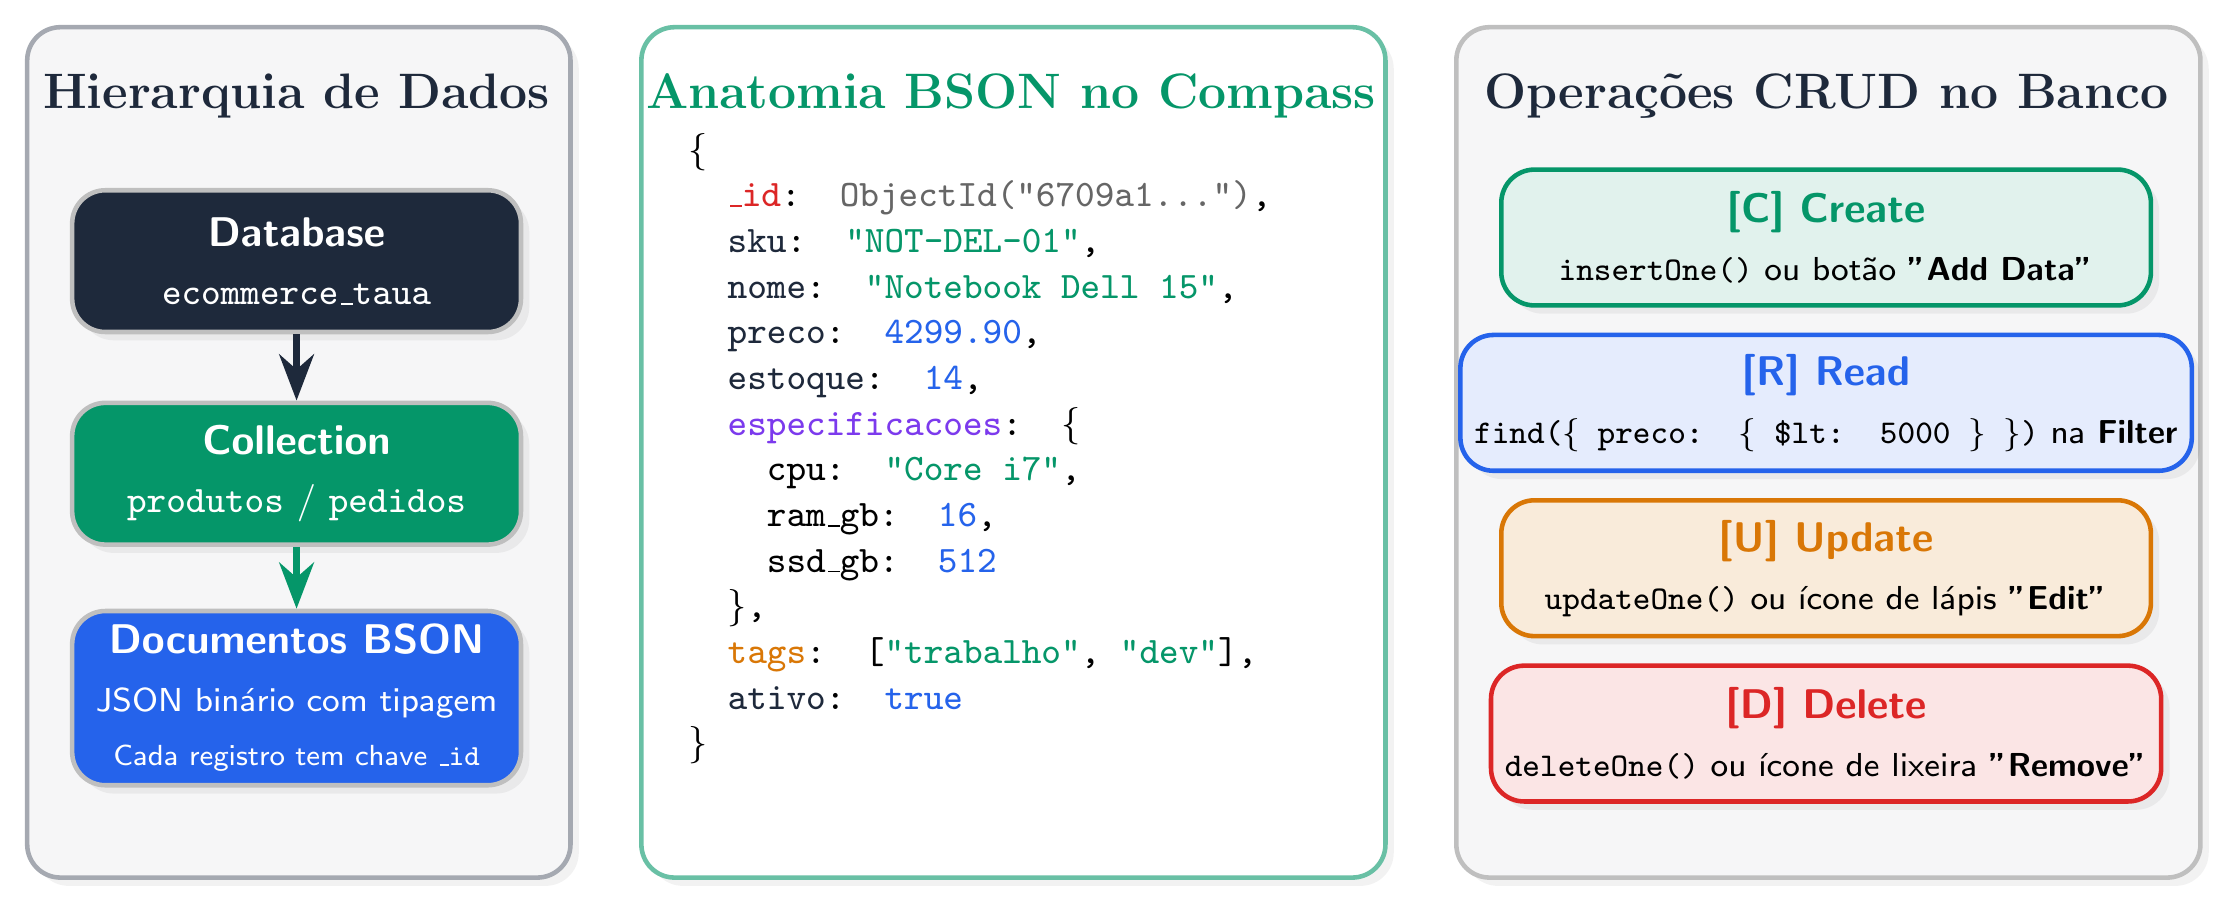
\includegraphics[width=0.98\textwidth,height=0.82\textheight,keepaspectratio]{figuras/fig_mongo_crud_compass.png}
\end{frame}

\begin{frame}{Operando no MongoDB Compass (Interface Gráfica)}
  \begin{columns}[T]
    \begin{column}{0.48\textwidth}
      \textbf{Passo a Passo Visual no Compass}
      {\footnotesize
      \begin{enumerate}
        \item Conectar em \texttt{localhost:27017} (ou Atlas).
        \item Criar banco \texttt{ecommerce\_taua} / \texttt{produtos}.
        \item Clicar em \textbf{Add Data} $\rightarrow$ \textbf{Insert Document}.
        \item Alternar para visualização \textbf{JSON} e colar.
        \item Clicar em \textbf{Insert} para persistir.
      \end{enumerate}
      }
    \end{column}

    \begin{column}{0.50\textwidth}
      \begin{block}{Consultas na Barra Filter}
        {\footnotesize
        \begin{itemize}
          \item \textbf{Filtro de Categoria:}\\
            {\scriptsize\texttt{\{ categoria: "Perifericos" \}}}
          \item \textbf{Filtro de Preço:}\\
            {\scriptsize\texttt{\{ preco: \{ \$lt: 1000 \} \}}}
          \item \textbf{Projeção} (\textit{Project}):\\
            {\scriptsize\texttt{\{ nome: 1, preco: 1, \_id: 0 \}}}
        \end{itemize}
        }
      \end{block}
    \end{column}
  \end{columns}
\end{frame}

\begin{frame}[fragile]{Terminal mongosh: Criação e Inserção Individual}
  \textbf{Seleção de Banco e Inserção com \texttt{insertOne}:}
\begin{lstlisting}[basicstyle=\ttfamily\scriptsize]
// 1. Criar e selecionar o banco de dados
use ecommerce_taua

// 2. Inserir documento individual rico com atributos aninhados
db.produtos.insertOne({
  sku: "NOT-DEL-01",
  nome: "Notebook Dell Inspiron 15",
  categoria: "Informatica",
  preco: 4299.90,
  estoque: 14,
  especificacoes: { processador: "Core i7", ram_gb: 16, ssd_gb: 512 },
  tags: ["trabalho", "desenvolvimento", "bivolt"],
  ativo: true
})
\end{lstlisting}
\end{frame}

\begin{frame}[fragile]{Terminal mongosh: Inserção em Lote (insertMany)}
  \textbf{Inserção Múltipla com Eficiência de Rede (\textit{Bulk Insert}):}
\begin{lstlisting}[basicstyle=\ttfamily\scriptsize]
db.produtos.insertMany([
  { sku: "MOU-LOG-02", nome: "Mouse Logitech MX",
    categoria: "Perifericos", preco: 589.00, estoque: 30 },
  { sku: "TEC-MEC-03", nome: "Teclado Keychron K2",
    categoria: "Perifericos", preco: 699.50, estoque: 20 },
  { sku: "MON-DEL-04", nome: "Monitor Dell 27 4K",
    categoria: "Monitores", preco: 2890.00, estoque: 8 }
])
\end{lstlisting}
  {\footnotesize
  \begin{itemize}
    \item Reduz \textit{round-trips} de rede agrupando registros em pacote único.
    \item Retorna um array com os \texttt{insertedIds} gerados automaticamente.
  \end{itemize}
  }
\end{frame}

\begin{frame}[fragile]{Terminal mongosh: Consultas Básicas e Projeção}
  \textbf{Filtros de Comparação e Seleção de Campos:}
\begin{lstlisting}[basicstyle=\ttfamily\scriptsize]
// 1. Buscar todos os documentos projetando apenas sku, nome e preco
db.produtos.find(
  {},
  { _id: 0, sku: 1, nome: 1, preco: 1 }
)

// 2. Filtrar produtos por categoria e preco menor que R$ 650 ($lt)
db.produtos.find({
  categoria: "Perifericos",
  preco: { $lt: 650.00 }
})
\end{lstlisting}
\end{frame}

\begin{frame}[fragile]{Terminal mongosh: Consultas em Arrays e Subdocumentos}
  \textbf{Busca em Estruturas Aninhadas (Dot-Notation):}
\begin{lstlisting}[basicstyle=\ttfamily\scriptsize]
// 1. Busca exata dentro de array de tags
db.produtos.find({ tags: "desenvolvimento" })

// 2. Consulta em objeto aninhado usando notacao de ponto
db.produtos.find({ "especificacoes.ram_gb": { $gte: 16 } })

// 3. Ordenacao decrescente por preco e limite
db.produtos.find().sort({ preco: -1 }).limit(3)
\end{lstlisting}
\end{frame}

\begin{frame}[fragile]{Terminal mongosh: Atualizações Atômicas e Remoção}
  \begin{columns}[T]
    \begin{column}{0.50\textwidth}
      \textbf{Modificações (\$set, \$inc, \$push)}
\begin{lstlisting}[basicstyle=\ttfamily\tiny]
// Atualizar preco e adicionar tag
db.produtos.updateOne(
  { sku: "NOT-DEL-01" },
  {
    $set: { preco: 3899.00 },
    $push: { tags: "liquidacao" }
  }
)

// Incrementar estoque de forma atomica
db.produtos.updateOne(
  { sku: "MOU-LOG-02" },
  { $inc: { estoque: 5 } }
)
\end{lstlisting}
    \end{column}

    \begin{column}{0.50\textwidth}
      \textbf{Deleção e Índices}
\begin{lstlisting}[basicstyle=\ttfamily\tiny]
// Remover documento individual
db.produtos.deleteOne({
  sku: "CAB-USBC-05"
})

// Remover produtos inativos
db.produtos.deleteMany({
  ativo: false
})

// Criar indice para busca veloz
db.produtos.createIndex({
  categoria: 1
})
\end{lstlisting}
    \end{column}
  \end{columns}
\end{frame}
